\documentclass[../main]{subfiles}
\begin{document}

\chapter{动目标检测及相参积累}%
\label{cha:mtd}

\section{实验报告}%
\label{sec:\arabic{chapter}report}

记录测试数据并填入表格,绘制特性曲线(线性/对数)

\begin{Answer}
  \begin{itemize}
    \item 波形见图~\ref{fig:mtd}。
    \item 对数幅频特性曲线见图~\ref{fig:mtd_}。
    \item 测试数据见表~\ref{tab:mtd}。
    \item 仿真代码见程序~\ref{lst:mtd}。
  \end{itemize}
\end{Answer}

\begin{figure}[htbp]
  \centering
  \begin{subfigure}[htbp]{0.45\linewidth}
    \centering
    \includegraphics[
      width = \linewidth,
    ]{images/mtd8.png}
    \caption{8 点动目标检测}%
    \label{fig:mtd8}
  \end{subfigure}
  \quad
  \begin{subfigure}[htbp]{0.45\linewidth}
    \centering
    \includegraphics[
      width = \linewidth,
    ]{images/mtd16.png}
    \caption{16 点动目标检测}%
    \label{fig:mtd16}
  \end{subfigure}
  \caption{动目标检测及相参积累}%
  \label{fig:mtd}
\end{figure}

\begin{figure}[htbp]
  \centering
  \begin{subfigure}[htbp]{0.45\linewidth}
    \centering
    \includegraphics[
      width = \linewidth,
    ]{figures/mtd8.pdf}
    \caption{8 点动目标检测}%
    \label{fig:mtd8_}
  \end{subfigure}
  \quad
  \begin{subfigure}[htbp]{0.45\linewidth}
    \centering
    \includegraphics[
      width = \linewidth,
    ]{figures/mtd16.pdf}
    \caption{16 点动目标检测}%
    \label{fig:mtd16_}
  \end{subfigure}
  \caption{对数幅频特性曲线}%
  \label{fig:mtd_}
\end{figure}

\begin{table}[htbp]
  \centering
  \caption{动目标检测}%
  \label{tab:mtd}
  \csvautobooktabular[respect percent]{tables/mtd.csv}
\end{table}

\langCVfile[matlab][lst:mtd][matlab]{figures/mtd.m}{figures/mtd.m}

\begin{Exercise}
  对实验中出现的现象进行分析说明。
\end{Exercise}

\begin{Answer}
  动目标检测是多个全等的脉冲平移不同距离后的叠加。
\end{Answer}

\begin{Exercise}
  实验报告中完成思考题。
\end{Exercise}

\begin{Answer}
  见章节~\ref{sec:\arabic{chapter}thought}。
\end{Answer}

\section{实验思考}%
\label{sec:\arabic{chapter}thought}

\begin{Exercise}
  为什么 FFT 等效于脉冲相参积累?
\end{Exercise}

\begin{Answer}
  因为傅立叶变换是多个延迟不同的横向滤波器的脉冲响应叠加。当输入信号与滤波器
  的特性曲线匹配时,输出响应达到最大,等效于脉冲相参积累。
\end{Answer}

\begin{Exercise}
  为什么要加权,如何选择窗函数?
\end{Exercise}

\begin{Answer}
  因为要抑制旁瓣电压,使能量集中在主瓣,从而让弱目标回波可以被检测出来。

  窗函数的主瓣宽度和副瓣电平是矛盾的。应综合考虑以选择合适的窗函数。
\end{Answer}

\begin{Exercise}
  FFT + MTI 方法实现 MTD 与 FIR 滤波器组实现 MTD 有何区别?
\end{Exercise}

\begin{Answer}
  \begin{itemize}
    \item FFT 在频域进行信号处理,输出延迟波形; FIR 在时域处理信号,输出实时
      波形。
    \item FFT 在零频附近凹陷不足,无法很好的抑制地物杂波,在 FFT 之前加上 MTI
      处理,先抑制地物杂波来改善检测性能。运算量少,速度快; FIR 可以灵活设计
      每个滤波器的权系数,使其幅度频率响应都在零频附近有较深的凹陷,用于抑制
      地杂波。具有灵活性高、运算控制简单,可根据杂波设计自适应和杂波抑制能力
      强等优点。
  \end{itemize}
\end{Answer}

\end{document}
